\documentclass[a4paper,10pt]{article}
\usepackage[margin=1in]{geometry}
\usepackage{graphicx}
\usepackage{amsmath}
\usepackage{listings}
\usepackage{xcolor}
\usepackage{pythonhighlight}
\usepackage{caption}  % Added for figure captions
\usepackage{setspace} % For line spacing
\usepackage{array} % For table formatting
\setstretch{1} % Reduce line spacing to 1

% Define colors for code
\definecolor{bg}{rgb}{0.95,0.95,0.95}
\definecolor{comment}{rgb}{0.5,0.5,0.5}
\definecolor{keyword}{rgb}{0.25,0.5,0.75}
\definecolor{string}{rgb}{0.5,0.25,0.25}

% Set up code listings
\lstset{
    backgroundcolor=\color{bg},
    basicstyle=\ttfamily,
    commentstyle=\color{comment},
    keywordstyle=\color{keyword},
    stringstyle=\color{string},
    breaklines=true,
    frame=single,
    tabsize=4,
    captionpos=b
}

\begin{document}
\vspace{-2cm}
\title{\LARGE \textbf{TRINITY COLLEGE DUBLIN} \\ % Reduced space between title and next line
\large School of Computer Science and Statistics}
\author{Abhishek Zade}
\date{} % Optionally remove date if not needed
\maketitle
\vspace{-1cm} % Adjust this value to reduce space between the author and title

\noindent
\textbf{StudentId:} 24332461 \hfill \textbf{Dataset id:} \# 17--34--17 \\
\textbf{Week 3 Assignment \hfill CS7CS4/CSU44061 Machine Learning} \\

% Horizontal line
\noindent\rule{\textwidth}{0.4pt} % This creates a horizontal line across the width of the page

\section*{Model Solution}

\subsection*{(i)}
\begin{enumerate}
    \item[(a)]   
In Figure 1, the 3D scatter plot of the data shows that the training points do not lie on a flat plane but instead follow a curved pattern, indicating a nonlinear relationship between the two features (X1, X2) and the target variable (Z-axis). The bending and dispersion of the points confirm that the data lies on a curve rather than a plane. This suggests that linear models may not fully capture the structure of the data, and higher-order polynomial features might be necessary for better modeling.
    \begin{center}
        \centering
        \includegraphics[width=0.75\linewidth]{week_3_a.1.png}
        \captionof{figure}{3D scatter plot showing nonlinear relationship}
        \label{fig:scatter-3d}
    \end{center} 
\newpage
\item[(b)] \textbf{Parameter from Lasso Model} \\
\begin{center}
        \centering
        \includegraphics[width=0.5\linewidth]{Screenshot 2024-10-11 at 3.35.28 PM.png}
        \captionof{figure}{Intercept Values for different Degree and C in Lasso Model}
        \label{fig:scatter-3d}
    \end{center} 
    
    As we can see from the above Figure 2 the Lasso regression results show how the model changes for various polynomial degrees (1 to 5) and values of the regularization parameter \( C \), where \( \alpha = \frac{1}{2C} \). As \( C \) increases, the influence of regularization decreases, allowing more complexity in the model. For lower degrees, such as 1 and 2, the coefficients are generally larger, resulting in simpler models. In contrast, higher-degree models (like 4 and 5) display more coefficients being reduced to zero, demonstrating Lasso's ability to encourage sparsity. The intercept remains consistent across models, but for higher \( C \) values (like 1000), fewer coefficients are shrunk to zero, indicating reduced regularization and greater flexibility in fitting the data. Overall, Lasso encourages simpler models with higher regularization, but larger \( C \) values enable more complex fitting.

\item[(c)] \textbf{Plot for Lasso Model (Prediction data Vs Original Data)}
\begin{center}
        \centering
        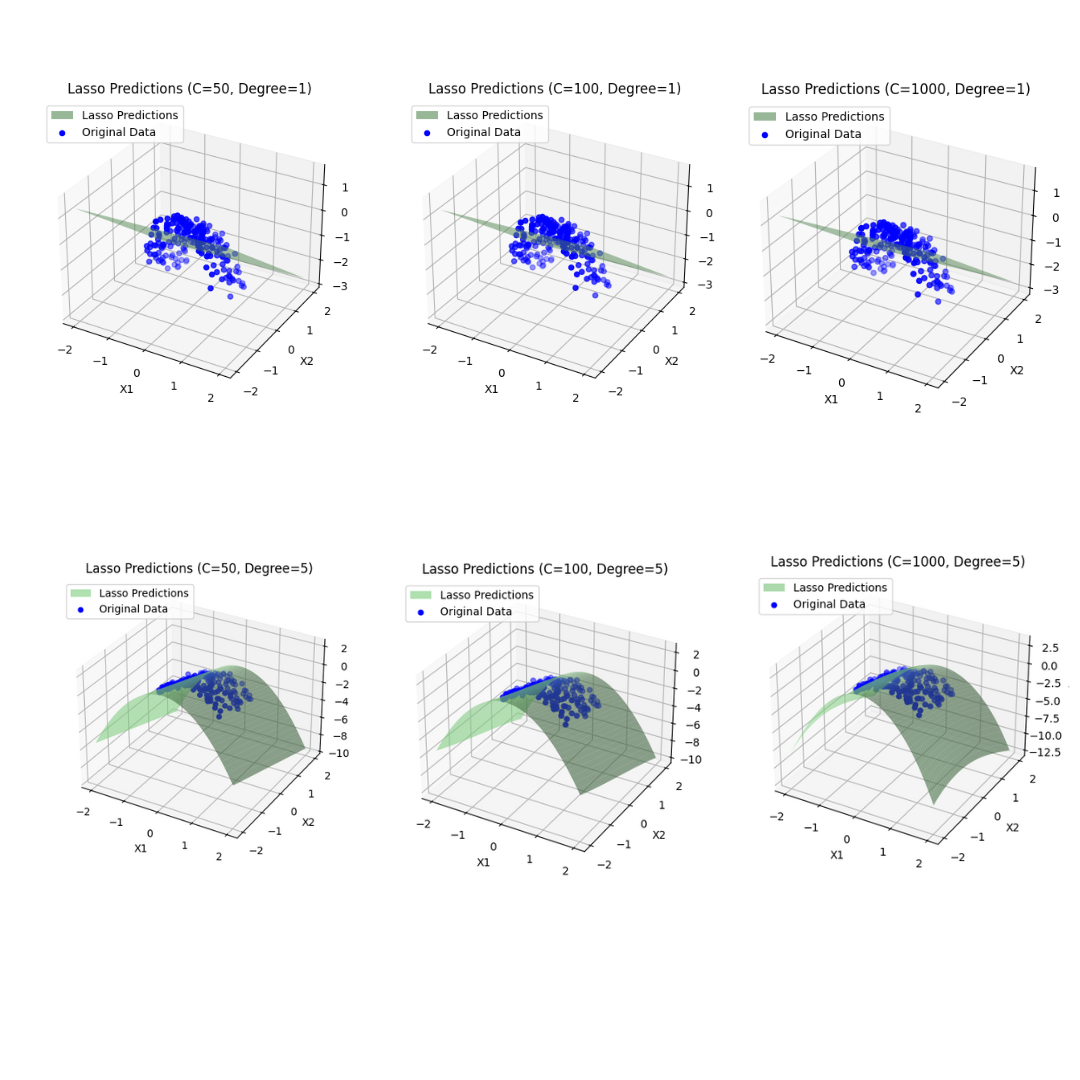
\includegraphics[width=0.75\linewidth]{3.png}
        \captionof{figure}{Lasso Model (Prediction data Vs Original Data)}
    \end{center}
    From \textbf{Figure 3}, we observe a variation in predictions when different values of \(C\) and polynomial degrees are used. In the upper half of \textbf{Figure 3}, we can see that when the degree is low, i.e., 1, the predictions form a linear surface. As \(C\) increases from 50 to 1000, the fit becomes slightly more responsive, but overall, when the degree is lower, the model remains rigid. We can say that for lower values of \(C\), regularization is strong, simplifying the model and making predictions less responsive to data variance. Now, when we look at the lower half of \textbf{Figure 3}, we can see that with a higher polynomial degree, i.e., 5, the model becomes more flexible or more responsive, and as \(C\) increases, i.e., towards 1000, regularization becomes much weaker. This allows the model to better fit the data, creating a more detailed curve. In general, we can say that higher \(C\) values reduce regularization, allowing more complex models to better fit the data, particularly for higher polynomial degrees.
\item[(d)]
A machine learning model is said to exhibit \textbf{underfitting} when the underlying model's algorithm is too simple to capture the complexity of the data. This leads to poor performance, especially when tested on complex data, as the model's predictions become inaccurate. To avoid underfitting, using a more complex algorithm within the model is recommended. Similarly, the model is said to be \textbf{overfitted} when it fails to make accurate predictions on testing data. This occurs due to an overly complex algorithm, which also captures noise in the data, leading to inaccurate predictions.

From \textbf{Figures 2} and \textbf{3}, we can conclude that a smaller $C$ leads to a larger penalty, resulting in a simpler model, and vice versa. Now, if we observe \textbf{Figure 3}, we can see that for a lower polynomial degree (i.e., 1), increasing $C$ results in similar predictions across different values of $C$, indicating that the model does not overfit easily for linear data. When the degree is higher (i.e., 5), the complexity is greater. With smaller $C$, more regularization leads to \textbf{underfitting}. For example, in \textbf{Figure 3}, when $C = 50$, observe the intercept at -0.075 and how the plot struggles to capture the data's shape, resulting in a simplified curve. As $C$ increases, the model becomes more stable, but increasing it too much leads to \textbf{overfitting}.

\item[(e)] \textbf{Lasso Model Vs Ridge Model}
\begin{center}
 \centering
        \includegraphics[width=0.5\linewidth]{Screenshot 2024-10-11 at 3.45.41 PM.png}
        \captionof{figure}{Intercept Values for different Degree and C in Ridge Model  }
        \label{fig:scatter-3d}
    \end{center} 
As compared to the Lasso model, in the Ridge model, no coefficients are reduced to exactly zero, even for higher degrees like 4 and 5. As \(C\) grows, the regularization weakens, and the model better fits the training data. We can observe in \textbf{Figure 5} that when the degree is higher, the Ridge model captures a wider area, even with a higher \(C\), compared to \textbf{Figure 3} for the Lasso model. The same is observed in \textbf{Figures 2 and 4}: the intercept when the degree is 5 and \(C = -0.0410\) for the Ridge model, and for the Lasso model when \(C = -0.075\), indicating more overfitting in the Lasso model for \(C = 50\), while the Ridge model appears to be more properly fitted.

    \begin{center}
\centering
        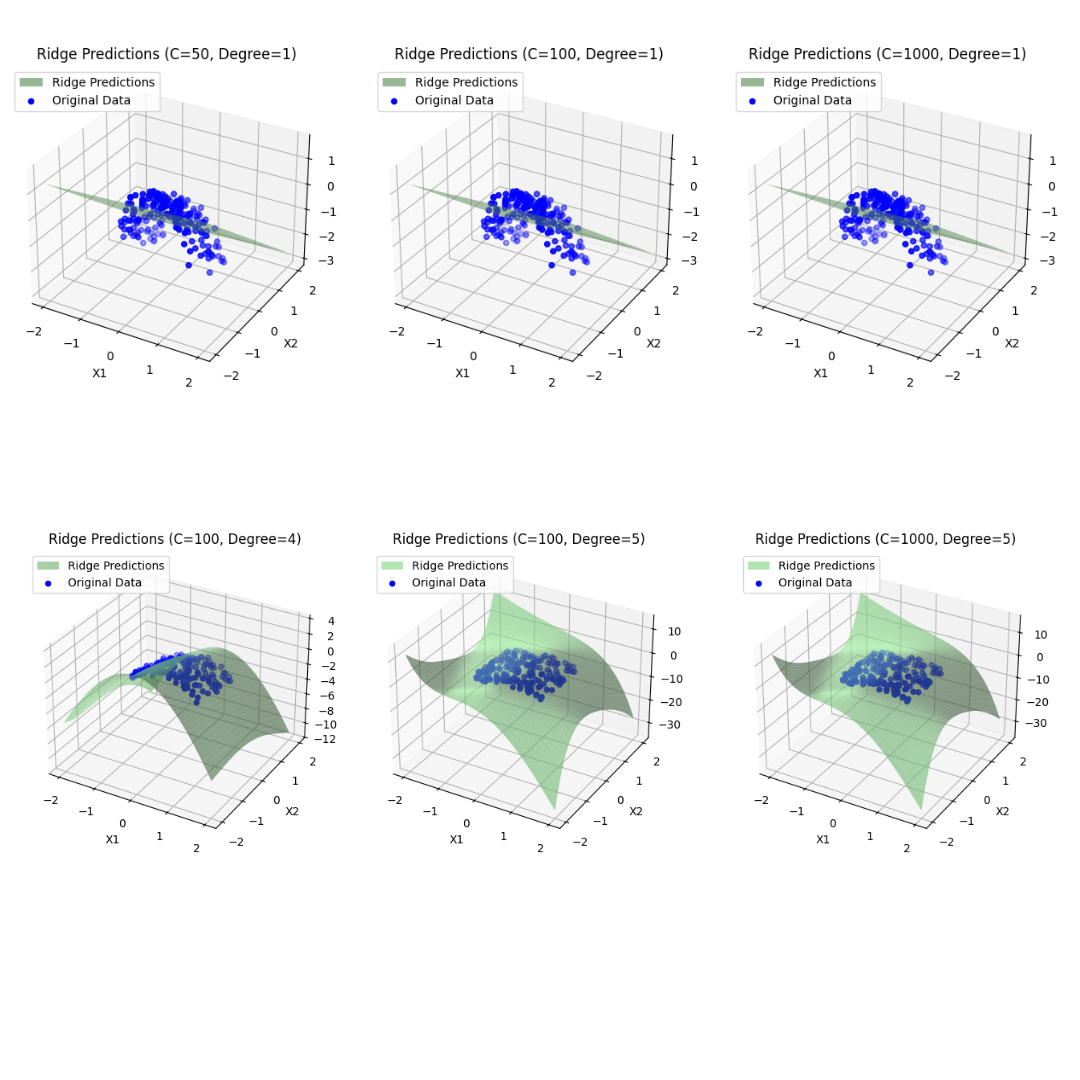
\includegraphics[width=0.75\linewidth]{4.png}
        \captionof{figure}{Ridge Model (Prediction data Vs Original Data)}
    \end{center}
\end{enumerate}
    \subsection*{(ii)}
\begin{enumerate}
\item [(a)]
 The range of values for \( C \) in the code is chosen to effectively demonstrate the impact of regularization on Lasso regression. The range \([0.01, 0.1, 1, 10, 100]\) covers a broad spectrum from strong to weak regularization. This allows for observing how the error decreases initially with increasing \( C \), indicating reduced overfitting. Beyond a certain point, the error stabilizes, showing that further decreasing regularization strength does not significantly affect performance. This range is practical for identifying optimal regularization levels in Lasso regression models.
 \newpage
    \item[(b)] \textbf{5-fold cross-validation (CV) Mean Error vs.  \textbf{\(C\)} for Lasso model}
     \begin{center}
\centering
        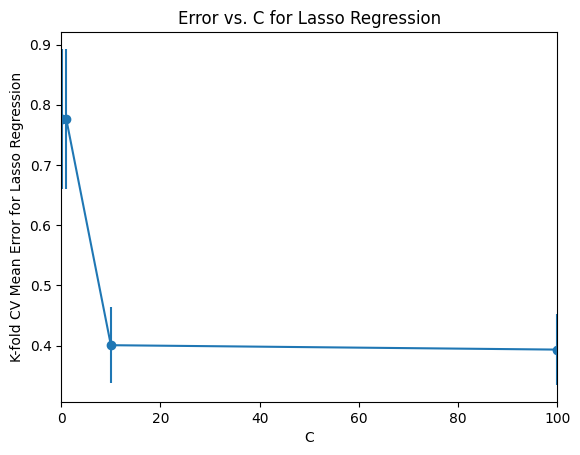
\includegraphics[width=0.75\linewidth]{2.1.1.png}
        \captionof{figure}{}
    \end{center}
    Based on the graph from \textbf{Figure 6}, I recommend using \textbf{\(C\) = 10} for Lasso regression. The cross-validation error decreases rapidly as C increases from 0.01 to 10 and then plateaus. After \(C\) = 10, there is no significant improvement in the error, indicating that higher values of \(C\) do not improve model performance. This choice of C balances the tradeoff between bias and variance, reducing underfitting without overly weakening the regularization effect. Therefore, \(C\) = 10 minimizes error while maintaining a reasonable level of regularization.
\item[(c)] \textbf{5-fold cross-validation (CV) Mean Error vs.  \textbf{\(C\)} for Ridge Model}
     \begin{center}
\centering
        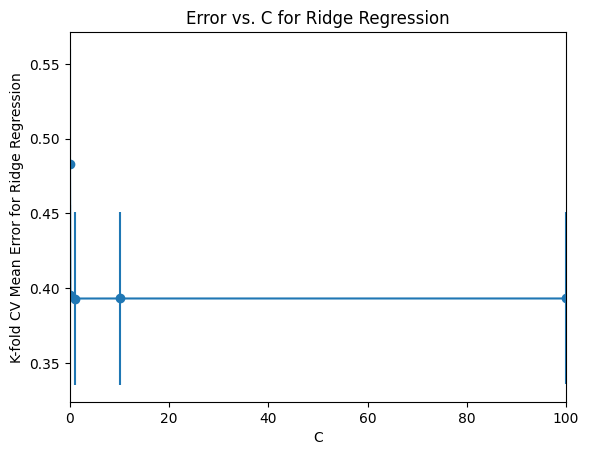
\includegraphics[width=0.75\linewidth]{2.1.2.png}
        \captionof{figure}{}
    \end{center}
    For Ridge regression, based on the graph from \textbf{Figure 7}, I recommend \textbf{\(C\) = 1}. The cross-validation error decreases initially but stabilizes at \(C\) = 1 and remains constant as \(C\) increases. Since higher values of \(C\) do not lead to significant error reduction, there is no benefit in choosing a larger \(C\). The model reaches its optimal error at \(C\) = 1, where regularization is balanced, preventing both underfitting and overfitting. Therefore, \(C\) = 1 minimizes error while keeping a sufficient level of regularization.
\section*{Appendix}
\begin{lstlisting}[language=Python, caption={}]
import numpy as np
import pandas as pd
import matplotlib.pyplot as plt
import matplotlib.lines as mlines
import matplotlib as mtplt
from mpl_toolkits.mplot3d import Axes3D
from sklearn.model_selection import train_test_split
from sklearn.linear_model import Lasso
from sklearn.linear_model import Ridge
from sklearn.preprocessing import PolynomialFeatures
from sklearn.model_selection import KFold
from math import sqrt

# id:17--34--17 
df = pd.read_csv("./data/week3.csv")
df.columns = ['X1', 'X2', 'y']
df.head()

X1 = df['X1']
X2 = df['X2']
X = np.column_stack((X1, X2))
y = df['y']
point = np.column_stack((X1, X2, y))

# (i) 
### (a)
fig = plt.figure()
ax = fig.add_subplot(111, projection='3d')
ax.scatter(X1, X2, y,color='blue', s=20, label='Original Data')
ax.set_xlabel('X1')
ax.set_ylabel('X2')
ax.set_zlabel('Y')
ax.set_title('Data Plot')
plt.show()

### (b) 
polynomial_values = [1, 2, 3, 4, 5]
result_list = []

for poly_degree in polynomial_values:
    poly_instance = PolynomialFeatures(degree=poly_degree)
    X_poly = poly_instance.fit_transform(X)
    X_train, X_test, y_train, y_test = train_test_split(X_poly, y, test_size=0.20, random_state=42)
    values_of_C = [1, 5, 10, 50, 100, 500, 1000]
    
    for C in values_of_C:
        lasso_reg = Lasso(alpha=1/(2*C))
        lasso_reg.fit(X_train, y_train)
        
        coef = np.around(lasso_reg.coef_, decimals=3)
        intercept = np.around(lasso_reg.intercept_, decimals=3)
        
        result_list.append({
            'Polynomial Degree': poly_degree,
            'C': C,
            'Coefficients': coef,
            'Intercept': intercept
        })

model_results = pd.DataFrame(result_list)

pd.set_option('display.max_colwidth', 600)

for poly_degree in polynomial_values:
    filtered_results = model_results[model_results['Polynomial Degree'] == poly_degree]
    
    styled_table = (
        filtered_results
        .style.set_table_styles(
            [
                {'selector': 'thead th', 'props': [('background-color', 'white'), ('color', 'black'), ('font-size', '12pt')]},
                {'selector': 'tbody td', 'props': [('background-color', 'white'), ('color', 'black'), ('border', '1px solid black')]},
            ]
        )
        .set_caption(f"Model results for Polynomial Degree {poly_degree}")
        .hide(axis='index')  # This hides the index
    )
    
    display(styled_table)



min_X = min(min(X1),min(X2)) - 1
max_X = max((max(X1),max(X2))) + 1
def kFoldModel(model_name):
    
    grid_range = np.linspace(min_X, max_X, 50)

    X1Test, X2Test = np.meshgrid(grid_range, grid_range)
    Xtest = np.c_[X1Test.ravel(), X2Test.ravel()]

    polynomial_values = [1, 2, 3, 4, 5]
    values_of_C = [1, 5, 10, 50, 100, 500, 1000]

    for poly_degree in polynomial_values: 
        poly_instance = PolynomialFeatures(degree=poly_degree)
        X_poly = poly_instance.fit_transform(X)
        X_poly_test = poly_instance.fit_transform(Xtest)

        for C in values_of_C:
            model_reg = None
            if(model_name == "Ridge"):
                model_reg = Ridge(alpha=1/(2*C))
            else:
                model_reg = Lasso(alpha=1/(2*C))
                
            model_reg.fit(X_poly, y)
            predictions = model_reg.predict(X_poly_test)
            Z = predictions.reshape(X1Test.shape)
        
            fig = plt.figure()
            ax = fig.add_subplot(111, projection='3d')
            surface = ax.plot_surface(X1Test, X2Test, Z, color='lightgreen', alpha=0.6, rstride=1, cstride=1)
            scatter = ax.scatter(X1, X2, y, color='blue', s=20, label='Original Data')
            surface_proxy = mlines.Line2D([0], [0], linestyle="none", color='lightgreen', marker='s', markersize=10)
            ax.legend([surface_proxy, scatter], [f'{model_name} Predictions', 'Original Data'], numpoints=1, loc='upper left')
            ax.set_xlabel('X1')
            ax.set_ylabel('X2')
            ax.set_zlabel('Y')
            ax.set_title(f'{model_name} Predictions (C={C}, Degree={poly_degree})')

            plt.show()
            
### (c) 

kFoldModel("Lasso")

### (e)
kFoldModel("Ridge")

# (ii)

def calulateErrorVsC(model_name):
    mean_error = []
    standard_deviation_error = []

    c_range = [1, 5, 10, 15, 25, 30, 40, 45, 100, 500, 1000]

    for C in c_range:
        model_reg = None
        if(model_name == "Lasso"):
            model_reg = Lasso(alpha=1/(2*C))
        else:
            model_reg = Ridge(alpha=1/(2*C))
            
        mean_square_error_array = []
        k_fold = KFold(n_splits=5)
        for train_index, test_index in k_fold.split(X):
            model_reg.fit(X[train_index], y[train_index])
            y_pred = model_reg.predict(X[test_index])
        
            # Calculate mean square error manually
            y_true = np.array(y[test_index])
            y_pred = np.array(y_pred)
            squared_diff = (y_true - y_pred) ** 2
            mean_square_error = np.mean(squared_diff)
            mean_square_error_array.append(mean_square_error)
    
        mean_error.append(np.mean(mean_square_error_array))
        standard_deviation_error.append(np.std(mean_square_error_array))

    plt.errorbar(c_range, mean_error, yerr=standard_deviation_error, fmt='-o')
    plt.xlabel('C')
    plt.ylabel(f'K-fold CV Mean Error for {model_name} Regression')
    plt.xlim((0, 55))
    plt.title(f'Error vs. C for {model_name} Regression')
    plt.show()


### (a)
calulateErrorVsC("Lasso")

### (c)
calulateErrorVsC("Ridge")

\end{lstlisting}

\end{document}
